
%(BEGIN_QUESTION)
% Copyright 2006, Tony R. Kuphaldt, released under the Creative Commons Attribution License (v 1.0)
% This means you may do almost anything with this work of mine, so long as you give me proper credit

Suppose an orifice plate is designed with a hole appropriately sized so that a water flow rate of 0 to 800 gallons per minute produces a differential pressure drop of 0 to 250 inches of water column.  Write the transfer function for this orifice plate, in terms of flow rate (Q), as determined by pressure drop ($\Delta P$).  In other words, write an equation with ``Q'' all by itself on one side of the = sign and $\Delta P$ on the other side, along with whatever operations and factors are necessary to make it work.

$$\includegraphics[width=15.5cm]{i00482x01.eps}$$

\underbar{file i00482}
%(END_QUESTION)





%(BEGIN_ANSWER)

$$Q = 50.596 \sqrt{\Delta P}$$

%(END_ANSWER)





%(BEGIN_NOTES)


%INDEX% Measurement, flow: orifice plate range calculation

%(END_NOTES)


